\documentclass[11pt]{article}

\usepackage[T1]{fontenc}
\usepackage[utf8]{inputenc}
\usepackage[english]{babel}

\usepackage[margin=1in]{geometry}
\usepackage{amsmath,amssymb,amsthm}
\usepackage{booktabs}
\usepackage[expansion=false]{microtype}
\usepackage{enumitem}
\usepackage{pgfplots}
\pgfplotsset{compat=1.18}
\usepackage[colorlinks=true,allcolors=blue]{hyperref}
\usepackage{listings}
\lstset{basicstyle=\ttfamily\scriptsize,breaklines=true,columns=fullflexible,
  keepspaces=true,showstringspaces=false,frame=single,framesep=3pt,
  xleftmargin=4pt,xrightmargin=2pt,aboveskip=4pt,belowskip=2pt}
\setlength{\emergencystretch}{3em}

\newtheorem{theorem}{Theorem}
\newtheorem{lemma}{Lemma}
\newtheorem{corollary}{Corollary}
\newtheorem{proposition}{Proposition}
\newtheorem{assumption}{Assumption}
\theoremstyle{definition}
\newtheorem{definition}{Definition}
\theoremstyle{remark}
\newtheorem{remark}{Remark}

\newcommand{\C}{\mathcal{C}}
\newcommand{\Cgood}{\C_{1}}
\newcommand{\Cbad}{\C_{0}}
\newcommand{\simF}{\sim_{F}}
\newcommand{\SigF}{\Sigma_{F}}
\newcommand{\SigN}{\Sigma_{N}}
\newcommand{\lF}{\lambda_{F}}
\newcommand{\lN}{\lambda_{N}}
\newcommand{\lst}{\lambda_{\mathrm{st}}}
\newcommand{\lred}{\lambda_{\mathrm{red}}}
\newcommand{\lirr}{\lambda_{\mathrm{irr}}}
\newcommand{\B}{\mathcal{B}}
\newcommand{\E}{\mathsf{E}}
\newcommand\blfootnote[1]{\begingroup\renewcommand\thefootnote{}\footnote{#1}\addtocounter{footnote}{-1}\endgroup}

\title{\vspace{-2em}Generated Gates Inherit Their Generator's Blind Spots:\\
\large A Diversity Floor for Self-Generated Verification}

\author{Ivo Matijašević\\ \small Independent Researcher \\ \small ivomatijasevic@gmail.com}
\date{June 2026}

\begin{document}
\maketitle
\blfootnote{\textcopyright~2026 Ivo Matijašević.\ This work is licensed under a Creative Commons
Attribution 4.0 International (CC BY 4.0) license, \url{https://creativecommons.org/licenses/by/4.0/}.}

\begin{abstract}
A growing body of empirical work reports that when language models generate the artifacts that
check other language models---unit tests, verifiers, evaluators, monitors---the checkers inherit the
generator's failure modes: machine-generated test suites mirror the generating model's error
patterns and miss the errors a human would make, model evaluators recognize and favor their own
outputs, and the self-preference extends to architecturally related model \emph{families}. We give a
representation-theoretic account of this phenomenon and prove two limits. Modeling a gate by the
indistinguishability relation of its underlying model family~$F$, with a \emph{stealth set} $\SigF$
of faults the family cannot separate from acceptable artifacts, we show \textbf{(GG1, inheritance)}
that any gate constructed within $F$ has a blind set containing $\SigF$---it cannot do better than
the family it is built from---and \textbf{(GG2, the self-generation floor)} that a closed system that
generates its own gates from a single founding family has an escape floor exactly equal to its
stealth mass $\lF=\mu(\SigF)$ (its blind set stabilizing at $\SigF$), a fixed point invariant to
generation depth, recursion, and prompt diversity. The floor is strictly
lowerable only by an \emph{exogenous} distinction source: a genuinely different family, whose
independent stealth set multiplies the floor down, or a reality-grounded gate that consults ground
truth rather than any family's representation and is the unique non-representational escape. The
results generalize the classical theory of coincident failures in $N$-version
programming~\cite{eckhardt1985,littlewood1989}---which assumed independently developed,
\emph{exogenous} versions---to the regime where the versions and their checkers are produced from
within one representational family, a regime that theory did not address; the new content is that
diversity cannot be bootstrapped from inside a family. We situate the floor as the origin of the
stealth mass that bounds verification in long-horizon agentic
work~\cite{matijasevic2026}, illustrate all claims in simulation, and state what must be measured to
make the floor quantitative for a given system.
\end{abstract}

\section{Introduction}
The dominant strategy for making unreliable generative systems usable is to check their outputs:
generate a candidate, then accept it only if it passes one or more gates---tests, static checks,
a second model asked to find fault, a panel of model judges. When the gates are good and disagree in
their mistakes, this works, and works quantitatively: a stack of imperfect but diverse gates can
drive the probability that a faulty artifact is accepted to an arbitrarily small
value, and can extend the reliable horizon of an unreliable executor without bound at overhead
logarithmic in the horizon~\cite{matijasevic2026}. The premise that does the work is
\emph{diversity}: the gates must not share the faults they miss.

It has become common to generate the gates the same way the candidates are generated---to write the
unit tests with the same model that wrote the code, to ask a model to critique its own output, to
build an evaluator panel out of one model family. The empirical record on this is now consistent and
unflattering. Machine-generated test suites exhibit tightly clustered error patterns and a
``homogenization trap,'' detecting the failures a model is prone to while missing the diverse
mistakes a human would make~\cite{homogenization2025}; verifiers built from such suites carry the
resulting blind spots and impose a ``verification ceiling'' on what they can
certify~\cite{verifceiling2025}; model evaluators recognize their own generations and score them
higher than human judges do, an effect causally tied to self-recognition~\cite{panickssery2024} and
traced to a familiarity preference for low-perplexity, self-like text, and the bias extends from the
individual model to its architectural \emph{family}~\cite{spiliopoulou2025}; and even heterogeneous
multi-agent teams have been observed to fail to match their single best member, with homogeneous
copies making matters worse~\cite{heteroteam2026}; and same-family model ensembles collapse to a
handful of effective voters, architectural kin sharing the very errors a calibrated vote then
amplifies~\cite{hiddenclones2026}. Each of these is an observation. What has been
missing is an account of \emph{why} it is a hard limit rather than a tendency to be engineered away,
and of exactly what \emph{can} escape it.

This paper supplies that account. We adopt the indistinguishability model that underlies the
diversity premise: a gate built from a model family can only act on distinctions that family can
represent, and is therefore blind to the faults that family confuses with acceptable artifacts. We
call that confusable-fault set the family's \emph{stealth set} $\SigF$ and prove two facts.

\begin{itemize}[leftmargin=1.4em,itemsep=2pt]
\item \textbf{Inheritance (Theorem~\ref{thm:gg1}).} Any gate constructed within family $F$ has a
blind set that contains $\SigF$. A generated gate cannot resolve a fault its generator cannot
resolve; it inherits the generator's blind spots.
\item \textbf{The self-generation floor (Theorem~\ref{thm:gg2}).} A closed system that generates its
own gates from a single founding family $F$---to any depth, with gates checking gates, under any
amount of prompt variation---has an escape floor exactly $\lF=\mu(\SigF)$. The floor is a fixed point
of the self-generation operator: it cannot be lowered from inside the family.
\end{itemize}

\noindent The floor is escapable, but only from outside. A gate from a genuinely different family $N$
has its own stealth set $\SigN\neq\SigF$; running it alongside the $F$-stack leaves only the faults
blind to both, of mass $\approx\lF\lN$ when the families are independent (Proposition~\ref{prop:exo}).
A \emph{reality-grounded} gate---one that decides by consulting ground truth, e.g.\ by executing the
candidate against a real oracle, rather than by any family's representation---can reject faults in
$\SigF$ on the scope its grounding covers, and is the unique escape that is not itself a
family (Proposition~\ref{prop:ground}). Neither route is available to a closed single-family system,
which is precisely the content of the floor.

\paragraph{Relation to prior theory.}
The inevitability of correlated failure among independently produced versions of a program is a
classical result. Eckhardt and Lee~\cite{eckhardt1985} showed that independent \emph{development}
does not yield independent \emph{failure}: because all versions are derived from one specification,
there is a nonzero set of inputs misinterpreted in a common way, and a ``difficulty function'' over
the input space induces positive failure correlation. Littlewood and Miller~\cite{littlewood1989}
extended this to \emph{forced} (methodological) diversity, proving that diverse development methods
can yield better-than-independent behavior. Knight and Leveson~\cite{knight1986,brilliant1990}
demonstrated the correlation empirically, as did the PODS experiment~\cite{bishop1988}; Hatton~\cite{hatton1997}
argued a single good version often outperforms $N$ diverse ones, and most recently $N$-version units
built from coding agents were found to fail coincidentally far above the independence
prediction~\cite{ron2026}. This theory was built for, and assumes, versions developed
by independent \emph{exogenous} agents---separate teams, separate methodologies. Our setting is the
one that theory did not consider: the versions, and the gates that check them, are produced from
within a single representational family, and the question is whether such a system can supply itself
the diversity Littlewood and Miller require. Theorem~\ref{thm:gg2} answers no. We recover the
classical results as the exogenous limit---a different family is methodological diversity realized in
representation space, and its effect is exactly the better-than-independent multiplication of
Proposition~\ref{prop:exo}---and add the impossibility of obtaining that diversity endogenously.
A companion analysis~\cite{matijasevic2026} shows that a shared stealth mass of size $\lst$ caps the
reliable horizon of gated long-horizon work at $\approx 1/\lst$ regardless of gate count; the present
paper identifies where that stealth mass comes from, why generated gates carry it, and what reduces
it (Remark~\ref{rem:n1}).

Two recent results bound self-correction by other routes. A diagonalization argument shows that every
enumerable model fails on some input, so a model correcting its own family inherits that existence
limit~\cite{fundlimits2025}; an information-theoretic bound constrains safety verification of
self-improving systems from finite observation~\cite{infotheoretic2026}. Our floor is complementary to
and orthogonal to both: a \emph{quantified} bound at the founding family's stealth \emph{mass}, located
in a family's representation rather than in computability or sample complexity, and---unlike an
existence or capacity limit---explicitly lowerable, by exogenous family diversity or reality-grounding.

\section{Model}\label{sec:model}
Fix a task with a ground-truth correctness predicate $\varphi$ on a space of candidate artifacts
$\C$. Write $\Cgood=\{c:\varphi(c)=1\}$ for the acceptable candidates and $\Cbad=\{c:\varphi(c)=0\}$
for the faulty ones. A faulty candidate that is accepted and promoted is said to \emph{escape}.
We measure faults with a fixed distribution $\mu$ on $\Cbad$ (the operative fault-generating
distribution); all masses below are $\mu$-masses, and ``$=$'' between fault sets may be read up to
$\mu$-null sets.

\begin{definition}[Gate and blind set]
A \emph{gate} $g$ is a decision procedure assigning each candidate a verdict in
$\{\textsf{accept},\textsf{reject}\}$. Its \emph{blind set} is the faulty mass it accepts,
$\B(g)=\{c\in\Cbad: g(c)=\textsf{accept}\}$. A stack of gates $G=\{g_1,\dots,g_k\}$ accepts a
candidate iff every gate accepts it, so a fault escapes the stack iff it lies in
$\bigcap_i \B(g_i)$; the stack's \emph{escape mass} is $\E(G)=\mu\!\left(\bigcap_i \B(g_i)\right)$.
\end{definition}

We require gates to be usable, i.e.\ to admit acceptable work: a gate has \emph{false-reject mass}
$\rho(g)=\nu\{c\in\Cgood: g(c)=\textsf{reject}\}$ under a distribution $\nu$ on $\Cgood$, and we
restrict attention to gates with $\rho(g)$ below a fixed tolerance $\rho_0$. (A gate that rejects
everything has empty blind set but is useless; the tolerance excludes it.)

\begin{definition}[Family and stealth set]\label{def:family}
A model \emph{family} $F$ has a fixed, finite parameter set; we characterize it by a \emph{representation
map} $r_F$ on $\C$ recording everything the family computes about a candidate \emph{across all of its
admissible prompt and scaffold configurations}, at $F$'s resolution. It induces the relation
$c\simF c'\iff r_F(c)=r_F(c')$: $c$ and $c'$ are indistinguishable to $F$ under \emph{every} prompt. As
the kernel of a map, $\simF$ is an equivalence relation (in particular transitive), and ``$F$ cannot
distinguish $c$ from $c'$'' means exactly $c\simF c'$. A gate is \emph{built within $F$}, or an \emph{$F$-gate}, if its
verdict is a function of the $\simF$-class of its input: it can only condition on what $F$ can
represent. The \emph{stealth set} of $F$ is
\[
  \SigF \;=\; \bigl\{\, c\in\Cbad : \exists\, c'\in\Cgood \text{ with } c\simF c' \,\bigr\},
\]
the faulty candidates that $F$ cannot separate from some acceptable candidate, with stealth mass
$\lF=\mu(\SigF)$.
\end{definition}

The relation $\simF$ is the formal carrier of ``what the family can tell apart.'' Because $r_F$ ranges
over all admissible prompt and scaffold configurations of a \emph{fixed} parameter set, Definition
\ref{def:family} makes a gate's discriminating power a property of its substrate, not of the prompt
wrapped around it: in-context learning and few-shot scaffolds navigate this fixed capacity---reweighting
what the parameters already compute---but cannot add a representational dimension the parameters and
training do not support, and $\SigF$ is exactly the intersection of the per-prompt blind spots over all
such configurations. This is the model assumption that does the work, and it is
the formal content of the empirical observation that self-preference is a family-level,
representation-level effect~\cite{spiliopoulou2025,panickssery2024} rather than a surface artifact.

\begin{remark}[Deterministic reduction of stochastic gates]
A stochastic gate---an LLM judge at temperature $T>0$---need not return a single verdict per candidate.
We take its verdict to be the deterministic reduction (greedy $T\to0$ decoding, or the thresholded
expectation $\mathbf{1}[\Pr(\textsf{accept}\mid r_F(c))\ge\tfrac12]$), which is a function of $r_F(c)$
and to which GG1--GG2 apply. Sampling variation at $T>0$ is then an additional false-accept/false-reject
noise source, folded into the tolerances and orthogonal to the representational blind set: re-rolling a
verdict cannot manufacture a distinction $r_F$ lacks, so it cannot reject a fault in $\SigF$.
\end{remark}

\section{Inheritance}\label{sec:gg1}

\begin{theorem}[GG1: generated gates inherit the generator's stealth]\label{thm:gg1}
Let $g$ be a \emph{sound} $F$-gate: $\rho(g)=0$ under a distribution $\nu$ that assigns positive mass
to every $\simF$-class meeting $\Cgood$. Then $\B(g)\supseteq\SigF$, and consequently
$\E(\{g\})\ge\lF$. More generally, suppose a \emph{uniform likelihood-ratio bound} holds: pushing
$\mu$ and $\nu$ forward to the space of $\simF$-classes (the faulty and good mass each class carries)
as $\bar\mu,\bar\nu$, one has $\mathrm{d}\bar\mu/\mathrm{d}\bar\nu\le\kappa$ on $\operatorname{supp}\bar\nu$
for a finite global $\kappa$. Then for $\rho(g)\le\rho_0$, $\B(g)\supseteq\SigF$ except on a stealth set
of mass at most $\kappa\rho_0$, which vanishes as $\rho_0\to 0$; absent such a finite $\kappa$, only the
sound case is claimed.
\end{theorem}

\begin{proof}
Let $c\in\SigF$. By definition there is $c'\in\Cgood$ with $c\simF c'$, so $g(c)=g(c')$ because $g$'s
verdict is a function of the $\simF$-class. If $g(c')=\textsf{accept}$ then $g(c)=\textsf{accept}$ and
$c\in\B(g)$; the only way $c\notin\B(g)$ is $g(c')=\textsf{reject}$, i.e.\ $g$ rejects the good part of
$c$'s class. For a sound gate ($\rho=0$) no good class of positive $\nu$-mass is rejected, so no such
$c$ exists and $\SigF\subseteq\B(g)$. For $\rho(g)\le\rho_0$, the rejected good classes carry total
$\bar\nu$-mass at most $\rho_0$; by $\mathrm{d}\bar\mu/\mathrm{d}\bar\nu\le\kappa$ their paired stealth
parts carry $\bar\mu$-mass at most $\kappa\rho_0$, so $\SigF\subseteq\B(g)$ off a set of mass
$\le\kappa\rho_0$. The escape bound
follows since $\B(g)\supseteq\SigF$ gives $\mu(\B(g))\ge\lF$.
\end{proof}

\begin{remark}[Generator versus substrate]\label{rem:substrate}
Theorem~\ref{thm:gg1} concerns the family on whose representation the gate \emph{decides}. A model of
family $F$ may \emph{author} a gate whose decisions are made by a different mechanism---a second
model, or an external tool---in which case the operative family is the deciding mechanism's, not the
author's. Two cases matter and are treated below: the deciding mechanism is another model family
(Proposition~\ref{prop:exo}) or it is a ground-truth oracle (Proposition~\ref{prop:ground}). A gate
both authored and decided within $F$---a checklist $F$ writes and $F$ applies, a model grading its
own family's work---is the case Theorem~\ref{thm:gg1} governs, and is the case that arises by default
when a system generates its own checkers.
\end{remark}

\section{The Self-Generation Floor}\label{sec:gg2}

We now consider a system that produces its own gates. A \emph{closed self-generating verification
system rooted in $F$} is any collection of gates obtained as follows: an initial set of $F$-gates,
together with any further gates produced by generators whose own decisions factor through $\simF$,
closed under such generation to arbitrary depth. The defining restriction is that no exogenous
representation enters: every gate in the closure, and every generator that produced it, is an
$F$-gate in the sense of Definition~\ref{def:family}. Let $\mathcal{G}_F$ denote the (possibly
infinite) set of gates reachable in such a closure, and let its escape floor be
$\E^\star_F=\inf\{\E(G): G\subseteq\mathcal{G}_F\}$, the least faulty mass any sub-stack drawn from
the closure can leave accepted.

\begin{theorem}[GG2: the self-generation floor is a fixed point at $\lF$]\label{thm:gg2}
For any closed self-generating verification system rooted in $F$,
\[
  \E^\star_F \;=\; \lF .
\]
The floor is invariant to generation depth, to gates checking gates, and to prompt diversity:
enlarging the closure by any amount of within-$F$ generation does not lower it. Equivalently, the
self-generation operator that maps a stack to any stack augmented with further $F$-gates fixes the
blind set at $\SigF$, hence the floor at $\lF$: it can neither go below it nor, with sufficient
within-$F$ coverage, fail to reach it.
\end{theorem}

\begin{proof}
\emph{Lower bound $\E^\star_F\ge\lF$.} A stack rejects a fault iff at least one of its gates rejects
it. By Theorem~\ref{thm:gg1}, every gate $g\in\mathcal{G}_F$ has $\B(g)\supseteq\SigF$ (for sound
gates; off a set of mass $\le\kappa\rho_0$ otherwise), so no gate in the closure rejects any fault in
$\SigF$. Hence $\SigF\subseteq\bigcap_{g\in G}\B(g)$ for every $G\subseteq\mathcal{G}_F$, giving
$\E(G)\ge\lF$ and therefore $\E^\star_F\ge\lF$.

\emph{Upper bound (achievability) $\E^\star_F\le\lF$.} Outside $\SigF$, every fault $c\in\Cbad
\setminus\SigF$ is, by Definition~\ref{def:family}, $\simF$-separated from all of $\Cgood$: its
$\simF$-class contains no acceptable candidate. An $F$-gate can therefore reject $c$ without any
false reject, and some $F$-gate does (a gate that rejects exactly the all-faulty $\simF$-classes is
an $F$-gate with $\rho=0$). Prompt and instance variation within $F$ ranges over such admissible
gates; a closure that includes, for each all-faulty class, a gate rejecting it has
$\bigcap_{g}\B(g)=\SigF$ and hence $\E(G)=\lF$. Thus the floor is attained.

\emph{Fixed point.} The two bounds give $\E^\star_F=\lF$. Augmenting any $G\subseteq\mathcal{G}_F$
with further $F$-gates cannot remove $\SigF$ from the intersection (lower bound) and cannot reduce
the floor below the already-attained $\lF$ (it is the infimum); the floor is therefore stationary
under within-$F$ generation. Depth, gates-checking-gates, and prompt diversity are all instances of
within-$F$ generation, since a generator whose decisions factor through $\simF$ produces only
$\simF$-measurable gates regardless of how it is prompted or composed.
\end{proof}

\begin{remark}[Why ``trying harder'' does not help]
Theorem~\ref{thm:gg2} is the formal statement that one cannot escape a family's blind spot by using
more of the same family. Generating a thousand tests with a model, having a model critique its own
critique, building a deeper panel of judges of one lineage, or searching over prompts---each is
within-$F$ generation and each leaves $\SigF$ exactly where it was. This is the limit behind the
empirically reported degeneration of single-model self-review into repetition of the original
error~\cite{homogenization2025,heteroteam2026}, now as a consequence rather than an observation.
\end{remark}

\section{Escaping the Floor}\label{sec:escape}

The floor is a statement about closed single-family systems. Two distinct moves leave the closure and
lower it.

\begin{proposition}[Exogenous family: independent stealth multiplies the floor]\label{prop:exo}
Let $N$ be a family with stealth set $\SigN$ and let a stack consist of an $F$-component that rejects
all faults outside $\SigF$ together with one $N$-gate that rejects all faults outside $\SigN$. The
stack's escape mass is $\mu(\SigF\cap\SigN)$. If the families' blind spots are independent under
$\mu$, $\mu(\SigF\cap\SigN)=\lF\lN$; in general $\mu(\SigF\cap\SigN)\le\min(\lF,\lN)$, with strict
reduction below $\lF$ whenever $\SigN$ does not contain $\SigF$. With $k$ families whose stealth sets
are mutually independent, the floor is $\prod_{i=1}^{k}\lambda_i$.
\end{proposition}

\begin{proof}
A fault escapes the stack iff every gate accepts it; the $F$-component accepts exactly $\SigF$ and the
$N$-gate accepts exactly $\SigN$, so the escaping set is $\SigF\cap\SigN$ with mass
$\mu(\SigF\cap\SigN)$. Independence gives the product; the bound
$\mu(\SigF\cap\SigN)\le\min(\lF,\lN)$ is monotonicity of measure; and if
$\SigF\not\subseteq\SigN$ then $\mu(\SigF\cap\SigN)<\lF$. The $k$-family statement is the same
argument on $\bigcap_i\Sigma_i$ under mutual independence.
\end{proof}

\noindent A different family is methodological diversity~\cite{littlewood1989} realized as
representational diversity, and Proposition~\ref{prop:exo} is its better-than-independent payoff. That
payoff is the \emph{independent} case $\mu(\SigF\cap\SigN)=\lF\lN$; independence of blind spots across
families is itself a strong, empirically checkable hypothesis---precisely the one Eckhardt and
Lee~\cite{eckhardt1985} showed independent \emph{development} does not by itself deliver---so it is the
joint mass $\mu(\SigF\cap\SigN)$, not the product, that a deployment must measure (\S\ref{sec:disc}).
The essential point for the floor is the hypothesis: $N$ must be \emph{exogenous}, $\SigN\neq\SigF$.
By Theorem~\ref{thm:gg2} a closed $F$-system cannot manufacture such an $N$; every gate it generates
has stealth $\supseteq\SigF$ and contributes nothing to $\SigF\cap\SigN$. Diversity that lowers the
floor must be imported, not bred.

\begin{proposition}[Reality-grounding: the non-representational escape]\label{prop:ground}
Let $h$ be a gate whose verdict is determined by a ground-truth oracle for $\varphi$ on a covered
scope $S\subseteq\C$---for instance, execution of the candidate against a real environment that
realizes $\varphi$ on $S$---and arbitrary off $S$. Then $\B(h)\cap S=\emptyset$: $h$ rejects every
fault in $S$, including faults in $\SigF$. Composing $h$ with an $F$-stack lowers the escape floor on
$S$ from $\SigF\cap S$ to $\emptyset$, leaving floor $\mu(\SigF\setminus S)$.
\end{proposition}

\begin{proof}
On $S$ the verdict of $h$ equals $\varphi$, so $h$ rejects every $c\in\Cbad\cap S$ and
$\B(h)\cap S=\emptyset$; in particular $\SigF\cap S\subseteq\Cbad\cap S$ is rejected by $h$
irrespective of $\simF$. The composed stack accepts a fault iff both accept it, so its escaping set is
$\big(\bigcap_g\B(g)\big)\cap\B(h)$, which on $S$ is empty and off $S$ is at most $\SigF$; the
residual floor is the un-grounded stealth $\mu(\SigF\setminus S)$.
\end{proof}

\noindent Reality-grounding is the one escape that is not itself a family: its discriminating power
comes from $\varphi$ directly, not from any $\sim$. It is the recovery-block acceptance test
of classical fault tolerance, here identified as the unique channel that imports
distinctions no representation supplies. Its reach is exactly its grounded scope $S$; the faults it
cannot escape are those that do not manifest under the available grounding, which is the genuine
specification-bound residue.

\begin{remark}[Decomposition of the stealth mass; relation to the horizon
bound]\label{rem:n1}
Write $\Sigma_{\cap}=\bigcap_i\Sigma_i$ for the intersection of the stealth sets of all families
\emph{available} to a system. Then a single family's stealth decomposes as
$\SigF=(\SigF\setminus\Sigma_{\cap})\uplus\Sigma_{\cap}$, matching the split of the stealth mass
$\lst=\lred+\lirr$ used in the long-horizon bound~\cite{matijasevic2026}: the
\emph{diversity-reducible} part $\lred=\mu(\SigF\setminus\Sigma_{\cap})$ is removed by importing
exogenous families (Proposition~\ref{prop:exo}), and the \emph{irreducible} part
$\lirr=\mu(\Sigma_{\cap})$---faults every available family confuses---is lowered only by
reality-grounding (Proposition~\ref{prop:ground}), down to the specification-bound residue no
grounding covers. The companion result then reads: the reliable horizon is capped at $\approx
1/\lst$, and the present paper says $\lst$ is a single founding family's $\lF$ for a self-generated
stack and falls only as exogenous families and grounding are added.
\end{remark}

\section{Numerical Illustration}\label{sec:num}
We illustrate the floor and its escapes in a transparent fault-population model (full code in the
appendix). A founding family $F$ has stealth mass $\lF=0.15$: a $0.15$ fraction of faults lie in
$\SigF$ and are invisible to every $F$-gate. On the remaining \emph{visible} faults each $F$-gate
fires independently with probability $q=0.6$. We measure the escape mass of (i) a tower of $h$
same-family gates, (ii) three different-prompt $F$-gates, (iii) the $F$-tower augmented with one
exogenous family-$N$ gate of independent stealth $\lN$, and (iv) the $F$-tower augmented with a
reality-grounded gate covering a fraction $g$ of the stealth faults. Each figure is a Monte-Carlo
average over $2\times10^{6}$ faults; reported values match the closed forms to sampling error. Arm
(iii) models the theoretical ideal of \emph{independent} blind spots (Proposition~\ref{prop:exo}); as
independence is the strong hypothesis flagged in \S\ref{sec:escape}, the appendix also reports a
correlated variant in which a shared cross-family bias $\rho_{FN}>0$ raises the floor strictly between
$\lF\lN$ and $\min(\lF,\lN)$---the regime a physical deployment occupies.

\begin{table}[h]
\centering
\small
\begin{tabular}{lcc}
\toprule
configuration & escape mass & closed form \\
\midrule
$F$-tower, depth $h=1$ & $0.490$ & $\lF+(1-\lF)(1-q)^h$ \\
$F$-tower, depth $h=3$ & $0.205$ & $\to\lF$ \\
$F$-tower, depth $h=8$ & $0.151$ & $\to\lF$ \\
$F$-tower, depth $h=15$ & $0.150$ & $\lF=0.15$ \\
three different-prompt $F$-gates & $0.205$ & floored at $\lF$ (prompt $\neq$ representation) \\
$F$-tower $+$ one exogenous $N$-gate ($\lN=0.15$) & $0.0225$ & $\lF\lN=0.0225$ \\
$F$-tower $+$ reality-grounded gate ($g=0.5$) & $0.075$ & $\lF(1-g)$ \\
$F$-tower $+$ reality-grounded gate ($g=0.9$) & $0.015$ & $\lF(1-g)$ \\
\bottomrule
\end{tabular}
\caption{The same-family tower plateaus at the founding stealth mass $\lF=0.15$ by depth $\approx 8$
and never falls below it (Theorem~\ref{thm:gg2}); prompt variation does not move it; only an
exogenous family (multiplying to $\lF\lN$, Proposition~\ref{prop:exo}) or a reality-grounded gate
(removing the grounded fraction, Proposition~\ref{prop:ground}) breaks the floor.}
\label{tab:num}
\end{table}

\begin{figure}[h]
\centering
\begin{tikzpicture}
\begin{axis}[
  width=0.72\textwidth, height=0.34\textheight,
  xlabel={stack depth $h$ (gates)}, ylabel={escape mass},
  xmin=1, xmax=15, ymin=0, ymax=0.55,
  legend pos=north east, grid=both, grid style={dotted},
  tick label style={font=\small}, label style={font=\small}, legend style={font=\small},
]
% same-family tower: lF + (1-lF)(1-q)^h, lF=0.15, q=0.6
\addplot[mark=o,thick,black] coordinates {
 (1,0.490)(2,0.286)(3,0.205)(4,0.169)(5,0.159)(6,0.154)(8,0.151)(10,0.150)(12,0.150)(15,0.150)};
\addlegendentry{same family $F$}
% F-tower + one independent N-gate, per added independent family the visible part also falls; floor lF*lN
\addplot[mark=square,thick,dashed,blue] coordinates {
 (1,0.245)(2,0.110)(3,0.061)(4,0.041)(5,0.032)(6,0.028)(8,0.024)(10,0.0228)(12,0.0225)(15,0.0225)};
\addlegendentry{plus exogenous family $N$}
% horizontal floor line at lF
\addplot[thick,red,dotted,domain=1:15] {0.15};
\addlegendentry{floor $\lambda_F=0.15$}
\end{axis}
\end{tikzpicture}
\caption{Escape mass versus stack depth. A same-family stack (solid) converges to the founding
family's stealth mass $\lF$ and stops; adding an exogenous family (dashed) moves the asymptote to
$\lF\lN$. No amount of within-family depth crosses the red floor.}
\label{fig:floor}
\end{figure}

\section{Discussion}\label{sec:disc}

\paragraph{What the floor does and does not say.}
The floor is about a family's blind set, not about model quality. A stronger model has a finer
$\simF$ and hence a smaller $\SigF$, so capability does shift the floor; what it cannot do is remove
the floor, and within a fixed family no amount of generation reaches below it. The result is therefore
orthogonal to the capability trend: better executors lower the founding floor, but only exogenous
diversity or grounding crosses it, and a self-generating system that lacks both is capped at its
founding family's stealth regardless of how capable that family is. This is the precise sense in which
``let the model check itself'' has a ceiling that scaling does not lift.

\paragraph{Consequences for self-improving verification.}
A system that improves its own checkers by generating new ones from its founding family improves
coverage of the faults it can already see and leaves $\SigF$ untouched; its escape floor is stationary
under self-improvement of the gate stack (Theorem~\ref{thm:gg2}). Lowering the floor requires adding a
distinction source the system does not already contain---another family, or reality-grounding---and
such a source must come from outside the self-generation loop, since by inheritance anything the loop
produces lies within $\SigF$. A design that economizes by replacing an exogenous checker with a
self-generated one of the founding family therefore raises the floor back to $\lF$ while appearing
to preserve the gate count: the loss is invisible to any measurement that does not track family
provenance. This floor is orthogonal to the \emph{collusion} failure studied in AI
control~\cite{greenblatt2024}, where an untrusted same-family monitor may \emph{intentionally} pass a
fault: the stealth floor binds even a perfectly honest monitor, since the blind spot is a limit of
representation, not of intent---and the two compound, a same-family checker being both blind and, if
misaligned, collusive.

\paragraph{What must be measured.}
The floor is quantitative only once $\SigF$ and the cross-family intersection $\Sigma_{\cap}$ are
measured. The blind set is not directly observable, but its mass is estimable from disagreement
statistics: faults that one family accepts and an exogenous family rejects bound $\SigF\setminus\SigN$
from below, and faults all families accept that a ground-truth probe later rejects estimate
$\Sigma_{\cap}$. Calibrating the pairwise stealth overlap as a function of representational distance
between families, and certifying that a candidate set of families has small joint stealth, are the
empirical companions to the theory; we leave their methodology to separate work and note only that the
theory tells one exactly which quantity---joint stealth across provenance-independent families---must
be driven down.

\paragraph{Limits of the account.}
Two assumptions bound the result. First, the model treats a gate's discriminating power as a function
of its family's representation; gates that combine a family with a tool or oracle are covered by
Propositions~\ref{prop:exo}--\ref{prop:ground} but a gate with idiosyncratic, non-family structure is
outside the model. Second, the stealth set is defined relative to a fixed correctness predicate
$\varphi$; where $\varphi$ is itself uncertain---the genuine specification gap---the ``faults'' a
family confuses with acceptable work are partly a property of the unresolved specification, and the
irreducible residue of Remark~\ref{rem:n1} inherits that uncertainty. Neither assumption affects the
two theorems, which are statements about a fixed $\varphi$ and a fixed family relation; they bound the
\emph{interpretation} of $\SigF$, not its consequences.

\section{Conclusion}
Diverse verification works because gates miss different faults; the question this paper settles is
where that diversity can come from. Within a single model family it cannot be generated: a gate built
from a family inherits the family's blind set (GG1), and a system that generates its own gates from
one founding family is capped at that family's stealth mass, a fixed point no depth, recursion, or
prompt variation lowers (GG2). The cap falls only when a distinction the family lacks is imported---a
genuinely different family, whose independent blind spot multiplies the floor down, or a
reality-grounded gate, whose verdict comes from ground truth rather than representation and which is
the unique non-family escape. The classical theory of coincident failures established that
independent development does not buy independent failure and that forced diversity helps; we have
shown, for the regime where the versions and their checkers are produced from within one family, that
the diversity forced diversity requires cannot be supplied from inside, and we have identified the two
exogenous sources that supply it. The practical reading is the one the recent empirical record keeps
arriving at: a system cannot verify its way out of its own blind spots, and what it needs is not more
of itself but something genuinely other---another family, or contact with reality.

\appendix
\section{Simulation code}\label{app:code}
The following self-contained script reproduces Table~\ref{tab:num} and the asymptotes of
Figure~\ref{fig:floor}. It models faults as stealth-to-$F$ (a fraction $\lF$, invisible to every
$F$-gate) or visible (each $F$-gate fires with probability $q$), and evaluates the same-family tower,
the prompt-diversity arm, the exogenous-family arm (independent and correlated), and the
reality-grounded arm against their closed forms.

\begin{lstlisting}[language=Python]
import numpy as np
rng = np.random.default_rng(7)

N        = 2_000_000   # faults sampled
lambda_F = 0.15        # founding-family stealth mass
q        = 0.6         # per-F-gate catch prob on a VISIBLE fault

stealth_F = rng.random(N) < lambda_F          # invisible to every F-gate

def F_tower_escape(h):
    """escape mass after h independent same-family-F gates."""
    if h == 0:
        return 1.0
    missed_visible = (rng.random((N, h)) > q).all(axis=1)
    return (stealth_F | (~stealth_F & missed_visible)).mean()

print("== same-family tower: plateaus at lambda_F, never below ==")
for h in [1, 2, 3, 5, 8, 15]:
    print(f"  h={h:2d}  escape={F_tower_escape(h):.4f}   (floor lambda_F={lambda_F})")

print("\n== prompt diversity within F: stealth set is a property of the")
print("   representation, not the prompt -> floor unchanged ==")
mv = (rng.random((N, 3)) > q).all(axis=1)
print(f"  3 different-prompt F-gates escape={(stealth_F | (~stealth_F & mv)).mean():.4f}")

print("\n== add ONE exogenous family-N gate (independent blind spot) ==")
for lambda_N in [0.15, 0.30]:
    stealth_N = rng.random(N) < lambda_N
    # big F-stack rejects all visible-to-F faults; survivors are stealth-to-F,
    # of which the N-gate rejects those it can see -> stealth-to-both remains
    print(f"  lambda_N={lambda_N}:  escape={(stealth_F & stealth_N).mean():.4f}"
          f"   (predicted lambda_F*lambda_N={lambda_F*lambda_N:.4f})")

print("\n== exogenous N with CORRELATION rho: independence (rho=0) is the ideal;")
print("   shared cross-family bias raises the floor toward min(lF,lN) ==")
lambda_N = 0.15
sd = (lambda_F*(1-lambda_F)*lambda_N*(1-lambda_N))**0.5
for rho in [0.0, 0.5, 1.0]:
    p_both = lambda_F*lambda_N + rho*sd            # target P(stealth in BOTH families)
    u = rng.random(N)
    stealth_N = np.where(stealth_F, u < p_both/lambda_F,
                                    u < (lambda_N - p_both)/(1 - lambda_F))
    print(f"  rho={rho}:  escape={(stealth_F & stealth_N).mean():.4f}"
          f"   (lF*lN={lambda_F*lambda_N:.4f}  min={min(lambda_F,lambda_N):.4f})")

print("\n== reality-grounded gate: rejects grounded fraction g of stealth faults ==")
for g in [0.0, 0.5, 0.9]:
    grounded_catch = rng.random(N) < g
    print(f"  g={g}:  escape={(stealth_F & ~grounded_catch).mean():.4f}"
          f"   (predicted lambda_F*(1-g)={lambda_F*(1-g):.4f})")
\end{lstlisting}

\begin{thebibliography}{99}

\bibitem{eckhardt1985} D.~E.~Eckhardt and L.~D.~Lee. A theoretical basis for the analysis of
multiversion software subject to coincident errors. \emph{IEEE Trans.\ Software Engineering}
SE-11(12):1511--1517, 1985.

\bibitem{littlewood1989} B.~Littlewood and D.~R.~Miller. Conceptual modeling of coincident failures
in multiversion software. \emph{IEEE Trans.\ Software Engineering} 15(12):1596--1614, 1989.

\bibitem{knight1986} J.~C.~Knight and N.~G.~Leveson. An experimental evaluation of the assumption of
independence in multiversion programming. \emph{IEEE Trans.\ Software Engineering}
SE-12(1):96--109, 1986.

\bibitem{brilliant1990} S.~S.~Brilliant, J.~C.~Knight, and N.~G.~Leveson. Analysis of faults in an
$N$-version software experiment. \emph{IEEE Trans.\ Software Engineering} 16(2):238--247, 1990.

\bibitem{bishop1988} P.~G.~Bishop. The PODS diversity experiment. In \emph{Software Diversity in
Computerized Control Systems}, Springer, 1988.

\bibitem{hatton1997} L.~Hatton. $N$-version design versus one good version.
\emph{IEEE Software} 14(6):71--76, 1997.

\bibitem{ron2026} J.~Ron, B.~Baudry, and M.~Monperrus. $N$-Version Programming with Coding Agents.
arXiv:2606.20158, 2026.

\bibitem{panickssery2024} A.~Panickssery, S.~R.~Bowman, and S.~Feng. LLM Evaluators Recognize and
Favor Their Own Generations. In \emph{Advances in Neural Information Processing Systems (NeurIPS)},
2024. arXiv:2404.13076.

\bibitem{spiliopoulou2025} E.~Spiliopoulou et al.\ Family-level self-preference bias in language-model
evaluators. 2025.

\bibitem{homogenization2025} Z.~Ma, T.~Zhang, M.~Cao, J.~Liu, W.~Zhang, M.~Luo, S.~Zhang, and
K.~Chen. Rethinking Verification for LLM Code Generation: From Generation to Testing.
In \emph{Advances in Neural Information Processing Systems (NeurIPS)}, 2025. arXiv:2507.06920.

\bibitem{verifceiling2025} M.~Thomas, T.~Partridge, et al.\ Verification Limits Code LLM
Training. arXiv:2509.20837, 2025.

\bibitem{heteroteam2026} Pappu et al.\ Heterogeneous multi-agent teams fail to match their best
member. arXiv:2602.01011, 2026.

\bibitem{hiddenclones2026} Z.~Bugaud. Hidden Clones: Exposing and Fixing Family Bias in
Vision-Language Model Ensembles. arXiv:2603.17111, 2026.

\bibitem{greenblatt2024} R.~Greenblatt, B.~Shlegeris, K.~Sachan, and F.~Roger. AI Control: Improving
safety despite intentional subversion. arXiv:2312.06942, 2024.

\bibitem{fundlimits2025} M.~A.~Mohsin, M.~Umer, A.~Bilal, et al. On the Fundamental Limits of LLMs
at Scale. arXiv:2511.12869, 2025.

\bibitem{infotheoretic2026} A.~Scrivens. Information-Theoretic Limits of Safety Verification for
Self-Improving Systems. arXiv:2603.28650, 2026.

\bibitem{matijasevic2026} I.~Matijašević. A Fault-Tolerance Threshold for Gated Agentic Computation:
Reliable Long-Horizon Work from Unreliable Executors. 2026. Preprint,
\url{https://doi.org/10.5281/zenodo.20837102}.

\end{thebibliography}

\end{document}
